\documentclass{article}

% Language setting
% Replace `english' with e.g. `spanish' to change the document language
\usepackage[english]{babel}

% Set page size and margins
% Replace `letterpaper' with `a4paper' for UK/EU standard size
\usepackage[letterpaper,top=2cm,bottom=2cm,left=3cm,right=3cm,marginparwidth=1.75cm]{geometry}

% Useful packages
\usepackage{amsmath}
\usepackage{graphicx}
\usepackage[colorlinks=true, allcolors=blue]{hyperref}
\usepackage[final]{pdfpages}
\usepackage{fancyhdr}
\usepackage{setspace}
\usepackage[shortlabels]{enumitem}
\usepackage{lastpage}

\onehalfspacing
\setlength{\parskip}{0.5\baselineskip}%
\setlength{\parindent}{0pt}%

\renewcommand{\headrulewidth}{.0mm} % header line width

\pagestyle{fancy}
\fancyhf{}
\fancyhfoffset[L]{1cm} % left extra length
\fancyhfoffset[R]{1cm} % right extra length
% \rhead{\today}
\lhead{\small Permanent Residence Petition for Mr. Wenbin Hu}
\rfoot{Page \thepage ~of \pageref*{LastPage}}

% \title{Your Paper}
% \author{You}

\begin{document}
% \maketitle

% \begin{abstract}
% Your abstract.
% \end{abstract}
\vspace*{\fill}
\begin{center}

{\bf 
Immigrant Petition for Alien Worker\\
for the Alien with Exceptional Ability in Science (EB2-NIW)
}

\end{center}
\vspace*{\fill}

\begin{center}
TABLE OF CONTENTS
\end{center}
\begin{itemize}
    \item [p. \pageref*{G-1145}] Form G-1145 e-Notification of Application/Petition Acceptance. 
    \item [p. \pageref*{I-140}] Form I-140, Immigrant Petition for Alien Worker with the \$700 filing fee.
    \item [p. \pageref*{I-907}] Form I-907, Request for Premium Processing Service with the \$2805 filing fee.
    \item [p. \pageref*{docs}] Photocopies of the passports, F-1 visas, Form I-20, Form I-94, EAD cards.
    \item [p. \pageref*{IE}] Initial Evidence in Support of the I-140 Immigrant Petition.
    \item [p. \pageref*{plans}] Statement from Mr. Wenbin Hu detailing plans on how he intends to continue work in the United States.
    \item [p. \pageref*{exhib}] Exhibits 1–30.
\end{itemize}

\clearpage
\label{G-1145}
\includepdf[pages=-,pagecommand={},width=1.3\textwidth]{./forms n docs/g-1145.pdf}

\label{I-140}
\includepdf[pages=-,pagecommand={},width=1.3\textwidth]{forms n docs/i-140.pdf}

\label{I-907}
\includepdf[pages=-,pagecommand={},width=1.3\textwidth]{forms n docs/i-907.pdf}

\vspace*{\fill}
\begin{center}

{\LARGE \bf
Title Page of the Current Passport
}
\label{docs}
\end{center}
\vspace*{\fill}

 
% \includepdf[pages=-,pagecommand={},width=1.3\textwidth]{forms n docs/Int Pass 27 Front Page.pdf}

\vspace*{\fill}
\begin{center}

{\LARGE \bf
The Current Student Visa (F-1)\\
in an expired passport
}

\end{center}
\vspace*{\fill}


% \includepdf[pages=-,pagecommand={},width=1.3\textwidth]{forms n docs/F1 2023.pdf}

\vspace*{\fill}
\begin{center}

{\LARGE \bf
Title Page of the Expired Passport\\
and expired US visas
}

\end{center}
\vspace*{\fill}


% \includepdf[pages=-,pagecommand={},width=1.3\textwidth]{forms n docs/Int Pass 23.pdf}

\vspace*{\fill}
\begin{center}

{\LARGE \bf
Current form I-20
}

\end{center}
\vspace*{\fill}


% \includepdf[pages=-,pagecommand={},width=1.3\textwidth]{forms n docs/SignedSTEM_I-20.pdf}

\vspace*{\fill}
\begin{center}

{\LARGE \bf
Current form I-94
}

\end{center}
\vspace*{\fill}


% \includepdf[pages=-,pagecommand={},width=1.3\textwidth]{forms n docs/I94.pdf}

\vspace*{\fill}
\begin{center}

{\LARGE \bf
Current Employment Authorization Document
}

\end{center}
\vspace*{\fill}


% \includepdf[pages=-,pagecommand={},width=1.3\textwidth]{forms n docs/EAD 2023.pdf}

\vspace*{\fill}
\begin{center}

{\LARGE \bf
Expired Employment Authorization Document
}

\end{center}
\vspace*{\fill}

.

% \includepdf[pages=-,pagecommand={},width=1.3\textwidth]{forms n docs/EAD 2022.pdf}



\begin{flushright}
Wenbin Hu\\
999 99th st,\\
Default City, FL, 99999\\
Tel. (999) 999-9999
\end{flushright}

December 31, 2024

\label{IE}
% Premium Processing
% USCIS Nebraska Service Center
% P.O. Box 87103
% Lincoln, NE 68501-7103

USCIS Nebraska Service Center\\
850 S. Street, Lincoln, NE 68508

\underline{\bf Initial Evidence in Support of the I-140 Immigrant Petition}

\begin{tabular}{ll}
{\bf Petitioner and Beneficiary:} & Mr. Wenbin Hu \\
{\bf Classification Sought:} & Employment-Based Immigration, Second Preference, \\
& Exceptional Ability in Science \\
& with a “national interest waiver” of the job offer (EB2-NIW).\\
& Sec. 203(b)(2)(B) INA [8 U.S.C. 1153].
\end{tabular}
\vspace{2\baselineskip}

Dear USCIS Officer,

This initial evidence is submitted in support of Mr. Wenbin Hu, M.Eng. in Control Engineering, who is filing the I-140 Immigrant Petition for Alien Worker. The evidence demonstrates that Mr. Hu is an individual of exceptional ability in the field of science, specifically in Medical Artificial Intelligence, and that his work will substantially benefit the national economy, educational interests, and welfare of the United States in the future.({\it Please refer to Sections 1, 2 and 3}).

Mr. Hu provides evidence that he satisfies three (A, D, F) of six criteria listed in 8 CFR, Section 204.5(k)(3)(ii), namely:
\begin{enumerate}
    \item Mr. Hu has an advanced degree in Control Engineering from a university in China. ({\it Please refer to Sections 1.1 and 3.2})
    \item Mr. Hu has commanded remuneration for his services, which demonstrates exceptional ability; ({\it Please refer to Section 1.2})
    \item Evidence of Mr. Hu's recognition for achievements and significant contributions to the field by peers and professional organizations. ({\it Please refer to Section 1.3})
\end{enumerate}
Due to the specifics of the highly-competitive area of Mr. Hu's occupation, Mr. Hu additionally provides evidence that he satisfies the following two (iv, vi) of ten criteria listed in 8 CFR, Section 204.5(h)(3) for determination of the extraordinary abilities. 
\begin{enumerate}
    \item Mr. Hu has participated, both individually and on a panel, as a judge of the work of others in the fields of Control Systems, Electrical Engineering, and Artificial Intelligence. ({\it Please refer to Section 1.4})
    \item Mr. Hu has authored scholarly articles in the fields of Control Systems, Cognitive Systems, and Artificial Intelligence. ({\it Please refer to Section 1.5})
\end{enumerate}

The criteria listed in 8 CFR, Section 204.5(h)(3) are comparable to the criteria listed in 8 CFR, Section 204.5(k)(3)(ii) due to the standards of exceptional ability being lower than the standard for extraordinary ability classification.

Mr. Hu is seeking a national interest waiver of the job offer, as per 8 USC 1153(b)(2)(B)(i) and 8 CFR  204.5(k)(4)(ii). The attached evidence and statement satisfy all three criteria for such a waiver, as described in Matter of Dhanasar, 26 I\&N Dec. 884 (AAO 2016). The supporting documentation and statement are as follows:

\begin{enumerate}
    \item Mr. Hu’s proposed work in Medical Artificial Intelligence has both substantial merit and national importance ({\it Please refer to Section 2})
    \item Mr. Hu is well-positioned to advance the proposed endeavor due to his expertise. ({\it Please refer to Sections 1 and 3})
    \item On balance, it would be beneficial to the United States to waive the job offer and labor certification requirements for Mr. Hu. ({\it Please refer to Sections 2 and 4, and Statement from Mr. Hu detailing plans on how he intends to continue work in the United States})
\end{enumerate}

In the United States, Mr. Hu plans to continue to work in the area of expertise. ({\it Please refer to the Statement from Mr. Hu detailing plans on how he intends to continue work in the United States and to Exhibits 8 and 9, his current job offers.})

Pursuant to 8 CFR, Section 204.5(k)(1), M.E Hu may file a petition on Form I-140 for classification under Section 203(b)(2) of the Act as an alien of exceptional ability in the sciences on his own behalf because he is seeking an exemption from the requirement of labor certification in the United States pursuant to Section 203(b)(2)(B) of the Act.

\clearpage

{\bf \underline{Section 1.} Mr. Hu is an alien of exceptional ability in the medical artificial intelligence who will prospectively substantially benefit the national economy, educational interests, and welfare of the United States.}

Mr. Hu's main area of study focuses on addressing a significant and pervasive health challenge: epilepsy and the unpredictable seizures it causes. By leveraging state-of-the-art computational techniques to predict seizures more accurately, the Beneficiary's research aims to enable proactive patient care, reduce the burden on the U.S. healthcare system, cut costs, improve quality of life for patients, and maintain the United States’ global leadership in medical innovation and biomedical engineering research. His planned endeavor is based on top of his past work and aims to advance these sub-fields even further.

 
{\bf 1.1 Mr. Hu has received degrees, including a B.Sc. degree in Electrical Engineering and Automation and a Master’s degree in Control Engineering  from high-ranking Universities. }

Mr. Hu obtained his Bachelor of Electrical Engineering and Automation and Master of Control Engineering Degree from the Hangzhou Dianzi University. ({\it Exhibit 8, Bachelor Diploma of Electrical Engineering and Automation, Exhibit 9, Master Diploma of Control Engineering.}) According to the ARWU Ranking 2024, it was near the top 3\%  best university in China (97/3074) and one of the Top 600 universities in the world. Specifically for the control automation professional ranking, the university is ranked top 150({\it Exhibit 10, Academic Ranking of World Universities 2024. Exhibit 11, Statistical Bulletin on the Development of National Education in China.}) 

His graduate-level performance was exceptional, achieving a high GPA (89.9/100) and ranking 4th out of 172 students, culminating in an “A” rating for his Master’s dissertation.({\it Exhibit 12, Graduate transcript.}) These academic achievements prove that he has mastered the complex theoretical framework of machine learning, signal processing, and artificial intelligence application principles.

{\bf 1.2. Mr. Hu has commanded a high compensation for services, demonstrating exceptional ability. }

When the applicant first graduated, the applicant was awarded an monthly salary of 17000 yuan at Huawei Technologies Co., Ltd. for his outstanding research.({\it Exhibit 13, Bank Revenue Flow 2019.}) Huawei is a top company in China and enjoys a certain reputation in the world. And compared to the average salary of a fresh graduate in 2019, the applicant's salary is 2.5 times that of a computer engineer (6,858 yuan/month), which is the highest paid in all field.({\it Exhibit 14, Salary of China's fresh graduates sees steady growth: report: https://english.www.gov.cn/news/topnews/202007/10/content_WS5f082574c6d06c4091250b16.html.})

After five years of employment, the applicant was recommended by the company to work in Hungary, where their total compensation exceeded 600,000 yuan. This total income is comprised of three components: the salary paid by the local Hungarian subsidiary, ({\it Exhibit 14, Subsidiary revenue proof, the currency is HUF, equal to xx yuan.}) the salary and benefits provided by the parent company,({\it Exhibit 15, Proof of Parent company's Income in 2024.}) and a stock dividend of 60,000 yuan.({\it Exhibit 16, Certificate of dividend income after tax, excluding 20 percent tax.}) The applicant's earnings are three times the average salary in the computer field for individuals with the same five years of experience, and significantly exceed the compensation in the highest-paying positions within the industry. ({\it Exhibit 16, Average survey for five years experiences employee in 2024.})

The illustrated major difference in Mr. Hu's compensation from the job market's standards comes from the competitive advantage that Mr. Hu has in the China job market due to his exceptional abilities in his fields of expertise. 

{\bf 1.3 Mr. Hu is recognized for achievements and significant contributions to the fields of Epileptic Seizure Prediction and Machine Learning by peers and professional organizations. }

{\bf 1.3.1 Other scientists recognize Mr. Hu’s exceptional knowledge of Epileptic Seizure Prediction and Machine Learning and consider Mr. Hu a top expert in these fields.}

Mr. Hu's international recognition is evident from the 6 letters supporting his petition that he received from six distinguished professionals from the China and abroad. ({\it Supporting Letters; Exhibits 2–7.}) 

All authors of supporting letters are recognized experts in the fields of Epileptic Seizure Prediction or Machine Learning. Three of them have been Mr. Hu’s mentors, while the other three have never worked with Mr. Hu directly but know his work from his publications and collaborative projects. 

“What sets Hu apart is his rare blend of technical expertise and applied problem-solving acumen. This unique skill set, which goes beyond standard engineering or data science competencies, is not easily replicated. The United States stands to gain substantially from his immediate and unrestricted involvement in ongoing research endeavors, clinical collaborations, and the development of next-generation medical devices.” ({\it Exhibit 4, letter from Mr. Xiangshao Liu})

“Through sophisticated CNN architectures and multi-layered deep learning frameworks, he has significantly improved the sensitivity and specificity of seizure prediction models we are developing. This improvement is not a marginal enhancement—it can fundamentally change clinical approaches to epilepsy management. By enabling preemptive intervention and careful resource allocation, these methods align seamlessly with U.S. objectives to enhance preventive care, mitigate chronic disease burdens, and reduce the overall financial strain on our healthcare system.” ({\it Exhibit 5, a letter from Professor D})

“The capacity to predict seizures before they occur is a transformative goal for neurology. By reducing unpredictability, we can lower emergency admission rates, refine treatment schedules, and empower patients with greater autonomy. The United States has invested extensively in health technologies that promote prevention, cost-effectiveness, and improved patient outcomes. Hu’s contributions exemplify these priorities, moving beyond traditional algorithms to extract previously inaccessible predictive insights from complex EEG signals.” ({\it Exhibit 7, a letter from Professor E.})

“Epilepsy management is an enduring challenge that consumes significant healthcare resources and often results in acute patient distress. By employing CNN-based deep learning methods to identify preictal EEG patterns with unprecedented accuracy, Hu has expanded our toolkit for anticipatory patient care. This improvement is no small feat. It reflects the kind of breakthrough that advances U.S. national interests in reducing healthcare expenditures, improving patient safety, and strengthening our capabilities in precision medicine.” ({\it Exhibit 6, a letter from Dr. D.})

{\bf 1.3.2 Mr. Hu has made original discoveries in Epileptic Seizure Prediction or Machine Learning. }

“Hu’s work in deploying stacked CNN architectures and refined feature extraction methods has substantially advanced our collective ability to forecast seizures. This step forward aligns seamlessly with national interests, as the U.S. healthcare system continually seeks innovative tools to improve patient care, minimize acute interventions, and contain escalating costs. His research directly supports these aims by turning complex EEG data into actionable clinical intelligence.” ({\it Exhibit 2, a letter from Professor Jiuwen Cao.}) 

“[...] Hu has made highly distinctive contributions to this field by integrating sophisticated Convolutional Neural Network (CNN) architectures, including stacked deep learning frameworks, to identify subtle preictal EEG biomarkers. His work, substantiated by peer-reviewed publications, not only surpasses conventional analytical approaches but also establishes new benchmarks for predictive accuracy and reliability.” ({\it Exhibit 3, a letter from Ms. Yibing Sheng.}) 

{\bf 1.3.3 Many scientists highly cite the papers co-authored by Mr. Hu. }

The significance and the impact of Mr. Hu’s work are demonstrated by the fact that his papers have been cited at least 187 times by xx research groups from the United States and other countries, according to citation reports from the Google Scholar citation database. ({\it Exhibit 18,Citation reports for Mr. Hu’s papers}) This number is constantly growing at rates higher than the impact factors of some of the corresponding journals. It is impressive for a young scientist who published his first paper merely 5 years ago when he was an graduate student. 

Mr. Hu’s papers have been cited by Professor H, the Vice Chancellor for Research and Distinguished Professor of Electrical Engineering and Computer Science at the University of H, by Prof. J, a professor of Machine Learning in the Computational and Biological Learning Lab, Department of Engineering, University of J, and Prof. K, a top researcher on Optimization in Machine Learning and AI, the Moorthy Family Professor in the departments of Mathematics, Statistics, and the Allen School of Computer Science and Engineering at the University of K.

“Previous research has shown promising results using con-volutional neural networks (CNNs) for epileptic seizureprediction. For example, Hu et al. used a CNN model andachieved an accuracy of 86.25% on the CHB-MIT dataset.The model demonstrated an improvement of nearly 12% inaccuracy for identifying preictal samples closer to a seizure,compared to those further in time. ” ({\it Exhibit 18, Citation reports for Mr. Hu’s papers})

“Other studies  used the raw EEG signals without any preprocessing and also achieved good results in predicting epileptic seizures. Besides, Cao and Hu et al. achieved multi level prediction of epilepsy and obtained good results using the Mean Amplitude Spectrum (MAS).” ({\it Exhibit 18, Citation reports for Mr. Hu’s papers})

"Epileptic EEG Classification Using Synchrosqueezing Transform with Machine and Deep Learning Techniques
The obtained results from the proposed ML-based methodand the DL-based method are promising compared with other recently published papers."  ({\it Exhibit 18, Citation reports for Mr. Hu’s papers})

"In our model, our fragment sampling adopts the method of [12,17], that is, 50% overlapping sampling of the data is performed to obtain the sampled data xZ ∈ R2 f , wheref is the sampling frequency, and then this fragment is used for feature extraction." ({\it Exhibit 18, Citation reports for Mr. Hu’s papers})

"Hence, by processing high-dimensional and combined EEG-fNIRS datasets, such DL algorithms have the potential to recognize intricate seizure patterns even when dealing with nonstationary or noisy data. For example, CNNs have proven to be effective for identifying and classifying EEG signals in [26]." ({\it Exhibit 18, Citation reports for Mr. Hu’s papers})

"To overcome these limitations, researchers have increasingly integrated manual feature extraction with deep learning techniques (Cao et al., 2019;Yuan et al., 2018). This combined approach leverages the strengths of both methods, enhancing model performance and accuracy in epileptic seizure detection and prediction." ({\it Exhibit 18, Citation reports for Mr. Hu’s papers})

"The subband mean amplitude of spectrum map (MAS) obtained from different EEG rhythms was adopted for EEG representation in [21], and stacked CNNs were used for feature extraction and seizure detection. It proved that the MAS has the ability to characterize the different rhythms of EEG signals. ..." ({\it Exhibit 18, Citation reports for Mr. Hu’s papers})

"For this purpose, firstly, we explore empirical mode decomposition (EMD) to decompose the EEG signal into intrinsic mode functions (IMFs), which are used via six statistical features as the input features of the brainwave classification for the character-writing application. Secondly, by getting inspired by [16,17] that the shallow learning classifiers provide the promising performance for the classification of binary classes, Gaussian mixture model (GMM) and kernel extreme learning machine (KELM) are applied to distinguish between a circle and straight line characters. Finally, the score combination of GMM and KELM is proposed to fuse the advantages based on different classifiers." ({\it Exhibit 18, Citation reports for Mr. Hu’s papers})


{\bf 1.4. Mr. Hu has been a judge of the work of others in the fields of Machine Learning and Artificial Intelligence. }

Mr. Hu has completed two peer review assignments from Journal of the Franklin Institute and AI MED journals, and has received invitations from two other journals, namely International Joint Conference on Neural Networks(IJCNN) 2025 and Association for the Advancement of Artificial Intelligence(AAAI) 2025. These are famous SCI journals and conferences in the field of artificial intelligence and engineering, for example, AAAI Conference on Artificial Intelligence is the \#4 venue in the ranking for Artificial Intelligence, which shows that hu's achievements are recognized by many journals.({\it Exhibit 20, Review assignments completed by Mr. Hu and review invatation by IJCNN and AAAI}) ({\it Exhibit 21, Journal Ranking for })


“[...] we have requested Mr. Hu’s expertise in the area of medical artificial intelligence under uncertainty to review the paper independently and provide feedback to the authors. The review was completed swiftly. Mr. Hu has made valuable suggestions allowing us to accept the manuscript after a revision, delivering an impact to the applications such as signal recovery with uncertainties in the sensing matrix and identification of parameters of time-invariant discrete-time linear dynamical systems via noisy observations.” ({\it Exhibit 22, A letter from Dr. XX, Editor of the AI MED jorunal}) 


{\bf 1.5 Mr. Hu is widely published in the fields of Computational Neuroscience and Artificial Intelligence. His publications have appeared in top journals in these fields.}

Mr. Hu has already published 2 peer-reviewed articles, and he also has a paper in the works, waiting to be published for peer review.. ({\it Exhibit 23, First pages of 3 papers co-authored by Mr. Hu.}) 

“Mr. Hu’s thesis results are published in prestigious venues as he made key experimental and intellectual contributions to many results produced in my group. Under my supervision, he has published 2 journal articles because of his key intellectual contribution to the work. Both of his journal articles are published in the top journals in the fields of Artificial Intelligence(Journal of Ambient Intelligence and Humanized Computing , top-xx h-index among open access journals) and Computational Neuroscience(IEEE Transactions on Cognitive and Developmental Systems, top-xx h-index overall).” ({\it Exhibit 2, a letter from Professor A.}) 

“The work with us is only a very small part of the Mr. Hu’s record since he has co-authored 2 papers before starting his work at our company. That is an impressive work, which summarizes well Mr. Hu’s commitment to his research. I consider myself very fortunate that he accepted to work on our research project.” ({\it Exhibit 3, Letter of Ms. Sheng})

According to the Google Scholar Metrics rankings of the venues in Artificial Intelligence and Computational Neuroscience, the journals and conferences that published papers by Mr. Hu are at the top of these fields by H-factor in 2023. ({\it Exhibit 24, Top venues rankings.}) For example, Journal of Ambient Intelligence and Humanized Computing is the top xx venue for publications on Artificial Intelligence, IEEE Transactions on Cognitive and Developmental Systems is the top-xx among the venues on Computational Neuroscienceg.

{\bf 1.6 Mr. Hu has performed a critical role in projects carried out for organizations of distinguished reputation. His knowledge and contribution to the fields have been invaluable to this job and have greatly impacted his area of study. }

“(From Cao)xx played an important role in the research team, not only completed its own research content outstandingly, but also completed the research beyond expectations with other team members, playing an indispensable role in the team.” ({\it Exhibit 2, a letter from Professor Cao.}) 

“Besides this paper, Mr. Hu co-authored several other high-profile papers during his work as a master student with his adviser Prof. Cao and colleagues from the Hangzhou Dianzi University. This distinction means that he was a key person in the published research and carried out most of the intellectual work.” ({\it Exhibit 7, a letter from Dr. C}) 

"(From Liu)Mr. Hu performs his duties as a engineer responsible for algorithms and software development at the AI+ Business Application Delivery Department of Huawei Technologies Co., Ltd. ({\it Exhibit 25, Employee Certificate of Incumbency.}) Huawei is one of the top Artificial Intelligence technology companies in the China. ({\it Exhibit 26, 12 Leading Chinese Companies in the AI Large Model Sector: https://equalocean.com/analysis/2023073019990.}) His responsibilities include researching machine learning models for predicting user behavior and intelligent conversations."

“(From Sheng)The optimization procedure was distributed over thousands of computational machines that had to work synchronously for many months, making the experiment extremely difficult to conduct from a technological point of view. This is where Mr. Hu applied his expertise, becoming responsible for the resiliency and robustness of the computational load to the potential issues coming from the unreliability of the underlying hardware and the limitations of the existing optimization algorithms used in modern AI training. Mr. Hu was surprisingly fast to onboard with the new team and worked collaboratively with our engineers which led to the successful completion of the planned experiments. [...] Working in our group, John has performed a key function and obtained hands-on experience in training large machine learning models that many believe to be the future of AI and the key to the next industrial revolution.” ({\it Exhibit 3, Letter of Ms. Sheng}) 


\clearpage


{\bf \underline{Section 2.} Mr. Hu’s proposed employment has both substantial merit and national importance for the United States.}
Mr. Hu intends to work in the fields of Epileptic Seizure Prediction and Machine Learning. The following descriptions of federal and state projects provide a summary of the importance and the urgency of the research in  Seizure Prediction:

{\bf 2.1 Epilepsy in the United States: A Pressing Public Health Challenge. }

Epilepsy affects approximately 3.4 million Americans, including nearly 3 million adults and 470,000 children, according to the Centers for Disease Control and Prevention (CDC). Characterized by recurrent seizures that occur unpredictably, epilepsy can result in injuries, hospitalizations, social stigma, and reduced quality of life. Patients and families often must navigate unpredictable episodes, impacting employment, education, and social integration.

Beyond the human toll, epilepsy imposes a significant economic burden. Healthcare costs related to epilepsy run into billions of dollars annually, including emergency room visits, hospital stays, long-term care costs, medications, and indirect costs related to lost productivity and disability. Interventions that reduce seizure frequency, severity, or unpredictability have enormous potential to alleviate these burdens.


{\bf 2.2 Why Seizure Prediction Matters. }

The unpredictability of seizures is a central challenge. Currently, treatments focus on reducing seizure frequency or severity through medications, surgical interventions, or devices like vagus nerve stimulators. But the unpredictable nature of seizure onset often remains. Patients cannot reliably know when a seizure will occur, which elevates risk, anxiety, and sometimes necessitates continuous care or supervision.

Accurate seizure prediction would be transformative. If patients could receive reliable warnings minutes or even seconds before a seizure, they could move to a safe space, prepare emergency medication, or contact support. Clinicians could personalize treatments based on an individual’s EEG profile, adjusting medication dosages or scheduling therapeutic interventions more effectively. This shift from reactive to proactive management aligns closely with U.S. healthcare goals emphasizing preventive care and patient empowerment.

{\bf 2.3 Why Seizure Prediction Matters. }

EEG is a cornerstone tool in epilepsy diagnosis and monitoring. EEG signals capture electrical activity in the brain, providing a non-invasive way to detect abnormal patterns that may herald a seizure. However, raw EEG data is notoriously complex, noisy, and high-dimensional. Human experts can interpret certain patterns, but subtle preictal states are often too subtle or variable to detect with conventional methods.
Machine learning, and deep learning in particular, excel at finding complex patterns in large datasets. CNNs have revolutionized image classification and speech recognition, and now they are being applied successfully to time-series biomedical data. By training CNNs on EEG recordings of patients who have seizures, these models learn to identify signatures that precede seizures. This leads to better accuracy, fewer false alarms, and earlier warnings.

{\bf 2.4 The Beneficiary’s Two Publications and Their Contribution to National Importance. }

1. First Publication in Journal of Ambient Intelligence and Humanized Computing (2023):
The Beneficiary’s initial study focused on mean amplitude spectrum-based epileptic state classification using CNNs. By extracting frequency-domain features (mean amplitude spectrum) and feeding these into CNN architectures, the research achieved more reliable classifications of EEG states, thereby improving the prediction of approaching seizures. This work laid the groundwork for integrating deep learning into clinical epilepsy care. The choice of mean amplitude spectrum features is not trivial—it reflects a deliberate engineering strategy to isolate features associated with imminent seizures. By sharing these results in a reputable international journal, the Beneficiary helped move the epilepsy research community closer to practical, AI-driven seizure prediction tools.

2. Second Publication in IEEE Access (2022): “Epileptic Signal Classification with Deep EEG Features by Stacked CNNs”:
The Beneficiary’s second paper ventured deeper into architecture innovation. He introduced stacked CNNs to learn deep EEG features, effectively capturing multi-scale temporal and spatial dynamics. While the first paper demonstrated that CNN-based classification is effective, the second paper showcased how architectural complexity and multi-layered feature extraction significantly enhance performance. Stacked CNNs can capture more intricate patterns, improving accuracy, sensitivity, and specificity of seizure detection and prediction. Published in IEEE Access, a respected platform known for rapid and open dissemination of peer-reviewed research, this work underscores the Beneficiary’s ability to pioneer more powerful and generalizable solutions. Such advancements are critical for clinical translation and are directly relevant to U.S. medical institutions seeking to integrate high-performing models into patient care.

Besides, the Beneficiary is still working in the group of Cao's group, and We continue to apply the latest technology to epileptic seizure detection, and cooperate with hospitals to apply algorithms to hospital data prediction. The latest algorithm based on xxx is proposed, which verifies the effect of Beneficiary's achievements on the public. These techniques can be applied to the relevant institutions of xx, thus having economic and practical help to xx, balabala.


Together, these two papers represent a trajectory of increasing sophistication, impact, and clinical relevance. They do not merely replicate known methods; they push the boundaries of what machine learning can do with EEG data, paving the way for widespread adoption in U.S. epilepsy care.

{\bf 2.5 Alignment with U.S. National Health and Research Priorities. }

The United States invests heavily in neurological research, often through NIH grants and other federal funding mechanisms. The NIH’s NINDS (National Institute of Neurological Disorders and Stroke) supports studies that improve diagnostics and treatments for epilepsy. Meanwhile, the NIH BRAIN Initiative encourages developing innovative tools and analytical methods to understand brain activity better and treat neurological conditions.

The Beneficiary’s research direction—a stronger, more precise method of EEG-based seizure prediction—resonates with these federal priorities. By improving prediction, we move closer to precision medicine in neurology, where treatments and interventions are tailored based on data-driven insights. This synergy with national strategies ensures that the Beneficiary’s work is not an isolated academic exercise, but directly relevant to ongoing federal and institutional efforts to advance neurological care.


{\bf 2.6 Economic and Strategic Implications. }

From an economic standpoint, breakthroughs in seizure prediction offer a path toward reducing the overall cost of epilepsy on the U.S. healthcare system. As healthcare models shift toward value-based care, interventions that prevent costly ER visits, hospitalizations, and complications align perfectly with national cost-containment and efficiency goals.

Strategically, the U.S. aims to remain a leader in medical AI and biomedical device innovation. Enhanced seizure prediction technologies can fuel the growth of American startups producing EEG-based wearables, telemedicine platforms, and hospital decision-support systems. These businesses would create jobs, attract global customers, and reinforce the U.S. as a hub of medical technology innovation. Thus, improvements in seizure prediction have a ripple effect extending well beyond direct patient care.

{\bf 2.7 Humanitarian and Ethical Dimensions. }

Improving epilepsy care is also a humanitarian imperative. Epilepsy patients often face stigma and constraints that limit their independence. Some cannot drive, work in certain industries, or fully participate in social life due to fear of unpredictable seizures. A reliable prediction tool can restore autonomy and dignity, enabling patients to manage their lives more freely. This aligns with American values of empowerment and equal opportunity.

In summary, the national importance of the Beneficiary’s research is evident at multiple levels: public health improvements, alignment with federal research priorities, economic benefits, strategic technological leadership, and ethical considerations that enhance patient well-being. These intersecting factors firmly anchor the Beneficiary’s work as having substantial merit and national importance.


\clearpage

{\bf \underline{Section 3.} The Beneficiary is well-positioned to advance the proposed endeavor due to his expertise. }

The second Dhanasar prong necessitates that the Beneficiary be well-positioned to advance his endeavor. This means he must have the skills, experience, credibility, and track record to move his research from theory to impactful application. The Beneficiary amply meets these criteria.


{\bf 3.1 Academic Excellence and Engineering Foundations.}

The Beneficiary’s advanced degree (Master’s in Control Engineering) from Hangzhou Dianzi University and high GPA highlight his capacity to master complex concepts. Control Engineering integrates mathematics, systems analysis, and signal processing—the perfect substrate for learning and implementing EEG data analytics. Ranking 4 out of 172 peers and earning an “Excellent” dissertation rating indicate that his professors and mentors recognized his abilities, analytical rigor, and research potential.

Such technical and theoretical competence is crucial, as EEG-based seizure prediction involves intricate pattern recognition, understanding signal theory, statistical modeling, and advanced algorithmic design. Without a strong theoretical grounding, it would be challenging to navigate the complexity of EEG signals and deep learning frameworks. ({\it Please see Exhibit 1, CV of Mr. Hu.}) 

{\bf 3.2 Comprehensive Research Experience in EEG-based Seizure Prediction.}

During his time in Professor Cao’s group, the Beneficiary engaged in full-stack EEG analytics. He did not specialize in just one facet; he learned to handle raw EEG signals, reduce noise, extract critical features, and implement machine learning pipelines. This hands-on immersion provided a holistic understanding of the challenges and solutions in epilepsy research.

He explored different machine learning models: CNN, SVM, KNN, and weighted fusion strategies. Such breadth ensured that he could compare models, tune hyperparameters, and integrate multiple architectures for optimal results. This versatility sets him apart from researchers who know only a single modeling approach. The Beneficiary can tailor solutions to diverse data sets and clinical conditions, a vital skill as no “one-size-fits-all” model exists for all EEG variations.


{\bf 3.3 Peer-Reviewed Publications Demonstrating Ongoing Innovation.}

First Paper (Journal of Ambient Intelligence and Humanized Computing):
Demonstrated the feasibility and improved accuracy of CNN-based seizure prediction using mean amplitude spectrum features. Publication in this reputable journal indicates that experts in the field found the methodology sound, the results credible, and the contribution meaningful.

Second Paper (IEEE Access – “Epileptic Signal Classification with Deep EEG Features by Stacked CNNs”):
Signifies a technical leap forward. By adopting stacked CNN architectures, he advanced from a baseline CNN model to a more complex and capable architecture that can learn deeper EEG representations. IEEE Access is known for thorough peer review and rapid dissemination, indicating that the Beneficiary’s work is cutting-edge, timely, and relevant.

These publications prove he is not only capable of conducting research but also of achieving recognized, peer-reviewed breakthroughs. Being first or among the early adopters of stacked CNN architectures for epileptic signal classification places him at the forefront of the field. ({\it Exhibit 4, a letter from Professor B.})

{\bf 3.4 Patent Application: Moving Toward Applied Innovations.}
His contribution to a Chinese patent application (No. 201810116608.9) related to CNN-based pre-seizure detection methods signals a transition from theory to innovation. Patents underscore novelty, utility, and potential commercial viability. By developing intellectual property, he shows readiness to contribute to medical device manufacturing, software solutions, and other commercial channels that could deliver immediate benefits to U.S. healthcare systems upon his involvement.


{\bf 3.5 Technical Skills: Programming, Software, and Documentation.}
The Beneficiary’s comfort with Python, data analysis libraries, Linux systems, and frameworks like TensorFlow ensures quick adaptation to U.S. labs and R\&D environments. Modern medical research relies heavily on open-source software stacks, version control systems, continuous integration, and reproducible machine learning pipelines. His ability to build TensorFlow models from source code if needed, run large-scale EEG data analyses efficiently, and document results thoroughly is essential for high-level collaborations.


{\bf 3.6 Interdisciplinary Expertise and Collaborative Potential.}
Epilepsy research is inherently multidisciplinary, blending neurology, clinical practice, biomedical engineering, signal processing, and machine learning. The Beneficiary’s profile—combining engineering foundations with deep learning advancements—makes him a valuable addition to U.S. teams that may already include neurologists, clinicians, data scientists, and hardware developers. He can communicate effectively across disciplines, aligning technical solutions with clinical realities.

{\bf 3.7 Access to U.S. Data and Resources.}
Once in the U.S., the Beneficiary could partner with NIH-funded epilepsy research consortia or collaborate with major institutions that have large EEG datasets. His methods, refined on these larger and more diverse data sets, could improve generalizability. This environment would let him iterate quickly, produce new models, and test them in clinical pilot studies. Such a fertile environment amplifies his ability to realize the full potential of his research.

In all these respects, the Beneficiary is undoubtedly well-positioned. He combines academic brilliance, proven research output, practical technical skills, and innovation-oriented thinking. He is not merely a student of the field; he is a contributor advancing the state of the art, as evidenced by his publications and patent application.


\clearpage

{\bf \underline{Section 4.} Benefit To The United States Of Waiving The Job Offer And Labor Certification Requirements. }

The third Dhanasar prong examines whether it is in the United States’ interest to waive the typical labor certification and job offer requirements. This section explains why the national interest would be best served by allowing the Beneficiary to proceed without these constraints.

{\bf 4.1 The Unique and Emerging Nature of the Work.}

Epileptic seizure prediction using advanced CNNs and deep EEG features is a specialized niche. While the U.S. workforce has many capable data scientists and engineers, relatively few possess the Beneficiary’s exact blend of EEG signal processing know-how, deep learning model design, and proven success in academic research and potential clinical translation. Labor certification requires defining a job in standard occupational categories and testing the market for U.S. workers. This works poorly when the job itself—interdisciplinary EEG-based seizure prediction research—is highly specialized and evolving. Waiting months or years for labor certification would stall urgent research efforts.

{\bf 4.2 Prompt Integration into Research and Healthcare Ecosystems.}

The Beneficiary’s work can have immediate applications in ongoing U.S. research projects. For instance, NIH-funded labs might currently be testing various seizure prediction algorithms. A startup developing wearable EEG monitors might be seeking a cutting-edge algorithm to differentiate itself and serve patients better. A major hospital system might be launching a clinical trial exploring AI-driven seizure management strategies. The Beneficiary, freed from the constraints of labor certification, can quickly join these efforts, maximizing impact and ensuring timely results. Any delay could mean missed opportunities to improve patient care or accelerate innovation.

{\bf 4.3 The High Value of Flexibility in National Interest Endeavors.}

The fundamental premise behind the National Interest Waiver is that certain endeavors surpass the benefits of a strict labor market test. Epilepsy research, improved seizure prediction, and the associated potential for cost savings and quality-of-life improvements meet this criterion. Granting the NIW allows the Beneficiary to choose collaborations and projects that yield the greatest national benefit rather than binding him to a single employer’s position. This flexibility ensures his skills can be allocated where they are most needed.


{\bf 4.4 Enhancing U.S. Global Competitiveness.}

Medical AI and neural engineering are hotly contested frontiers. Countries worldwide are racing to attract top talent. If the Beneficiary is hampered by the labor certification process, he might pursue opportunities elsewhere. By granting the NIW, the U.S. secures a researcher who can help maintain and even extend the nation’s leadership in medical technology. The global healthcare AI market is expanding rapidly, and the U.S. stands to gain from having leading experts developing next-generation solutions domestically.


{\bf 4.5 Reducing Healthcare Costs and Improving Patient Outcomes.}

By enabling better seizure predictions, the Beneficiary’s work can reduce unnecessary healthcare expenses. Fewer emergency admissions mean lower costs for hospitals, insurers, patients, and government programs like Medicare and Medicaid. Over time, the widespread adoption of advanced seizure prediction models could translate into billions saved, aligning perfectly with U.S. goals of cost-effective, high-quality healthcare.


{\bf 4.6 Legislative Intent and the Nature of National Interest Waivers.}

National Interest Waivers are intended for cases precisely like this, where a labor market test adds little value and may hinder significant national benefits. The Beneficiary’s research direction is not a commodity skill set. By approving the NIW, USCIS would fulfill the spirit of the relevant statutes and decisions (Dhanasar and prior precedents), facilitating the admission of individuals whose expertise and contributions are vital to national interests.

{\bf 4.7 No Detriment to U.S. Workers.}

It is important to recognize that granting an NIW Hu's not harm U.S. workers. The specialized nature of the Beneficiary’s work means he complements existing teams rather than replacing or undercutting them. His arrival could create more opportunities as his research leads to new projects, funding, and technology developments. Ultimately, enhanced epilepsy care benefits not only patients but also the broader economy and the healthcare industry at large.

In essence, the balancing test strongly favors waiving the labor certification requirement. The U.S. gains immediate and flexible access to a uniquely qualified researcher who can advance a nationally significant area of healthcare research and innovation.

\clearpage

{\bf \underline{Section 5.} Concluding Remarks. }

""
“Clearly, Mr. Hu is an exceptionally talented mathematician and engineer, and he would be a great asset to the United States if he continued working here. If he enters academics as a Engineer, as planned, then he will make important contributions to the medical artificial intelligence for State and the US, training future generations of engineers among the Veterans and the native population. If he stays in the industry, he will create new commercial opportunities based on his advanced knowledge of next-generation AI technology and the safety of large computational systems. In short, Mr. Hu is already a leader in main areas of immense importance to our economy and national security, and his leadership position will inevitably increase. Please give favorable consideration to his Green Card application.” ({\it Exhibit 2, a letter from Professor A.}) 

“I endorse the immigration petition by Mr. Hu and ask you to decide favorably on his behalf so that he can continue his important research without delays and distractions.” ({\it Exhibit 4, a letter from Professor B.}) 

"Mr. Hu offers a unique skillset to the American scientific community. He is a creative engineer with an unusually keen attention to detail. I strongly support his application." ({\it Exhibit 3, a letter from F.}) 

“Let me finish this letter with the statement that Mr. Hu is a brilliant young investigator in the fields of operations research and artificial intelligence. Granting him permanent residence in the U.S. will allow his work to proceed uninterrupted so he can concentrate on the application of his skills and knowledge to solving major computational problems.” ({\it Exhibit 5, a letter from Dr. C.}) 

“I wholeheartedly endorse Mr. Hu's application for the EB-2 NIW petition for Permanent Residence. His advanced research and demonstrated leadership in his field make him a strong candidate, and I am confident that his ongoing contributions will substantially benefit our nation.” ({\it Exhibit 7, a letter from Professor E.}) 

“In my opinion, Mr. Hu has made very significant discoveries in control and signal processing and helped in the advance of operations research. His outstanding abilities and expertise will be a huge asset to the science of computation in the USA. There is no doubt he will continue to have a major impact on electrical engineering, operations research, machine learning, and artificial intelligence. He will certainly contribute substantially to the well-being of American society and help sustain the USA as the leading light in world science.” ({\it Exhibit 6, a letter from Dr. D.}) 

The Beneficiary’s research into EEG-based epileptic seizure prediction using advanced machine learning techniques, including stacked CNNs, directly addresses a critical national interest. By tackling a major healthcare challenge—epilepsy—and offering solutions that could improve patient independence, reduce healthcare spending, and enhance U.S. leadership in medical AI, his work holds substantial merit and national importance.

He has demonstrated, through exemplary academic performance, hands-on research experience, two peer-reviewed international publications, and a patent application, that he is eminently well-positioned to advance this field. He is not a novice but a researcher who has already achieved innovations recognized by the international scholarly community.

Requiring a job offer and labor certification would slow the pace of beneficial collaborations, limit his potential contributions, and ultimately serve as an unnecessary barrier to harnessing his specialized skill set for the U.S. public good. Granting a National Interest Waiver aligns perfectly with the legislative intent behind the NIW category and ensures that his talents can be immediately and fully leveraged to advance public health and scientific innovation in the United States.

For these reasons, I respectfully request that USCIS approve this petition and grant the National Interest Waiver for the Beneficiary. Should there be any need for additional information or clarification, I will be pleased to provide further documentation.
Thank you for your time and careful consideration.

Respectfully submitted,

\vspace{5\baselineskip}

Wenbin Hu\\
999 99th st,\\
Default City, FL, 99999\\
Tel. (999) 999-9999




\clearpage

{\bf Statement from Mr. Hu detailing plans on how he intends to continue work in the United States}

\label{plans}
December 31, 2024

My name is Wenbin Hu. I am writing this letter to provide a detailed overview of my plans on how I intend to continue my research and related endeavors in the United States, should my National Interest Waiver (NIW) petition be approved. As outlined in my I-140 petition, my area of focus is improving the prediction and understanding of epileptic seizures through advanced EEG-based machine learning techniques. By bringing my expertise to the U.S., I aim to drive meaningful progress in epilepsy care, contribute to medical AI innovation, and engage with various American institutions and enterprises dedicated to this field.

Below, I present my strategic approach and anticipated activities, collaborations, and contributions, reflecting how I envision establishing myself as a productive and influential researcher in the United States.


{\bf 1. Academic and Clinical Collaborations }

{\bf University Partnerships: }

I plan to affiliate with leading academic medical centers and universities known for epilepsy and neuroscience research, such as Johns Hopkins University, the Mayo Clinic, and the Cleveland Clinic. Working within their neurology and biomedical engineering departments will provide access to large EEG datasets and ongoing clinical trials. This environment will allow me to validate my algorithms against diverse patient populations, refine predictive accuracy, and rapidly incorporate clinical feedback.

{\bf NIH and NINDS Initiatives: }

I aim to align my work with NIH-funded projects, including initiatives by the National Institute of Neurological Disorders and Stroke (NINDS), and possibly the BRAIN Initiative. By joining consortia focused on improving diagnostic and therapeutic approaches for epilepsy, I can integrate my models into federally supported research, ensuring my contributions directly advance U.S. public health goals.

{\bf 2. Industry and Startup Engagement }

{\bf Medical Device Firms and AI Companies: }

The U.S. has a thriving healthcare technology sector. I will seek collaborations with startups and established med-tech companies developing EEG-based monitoring devices or AI-driven healthcare platforms. Integrating my seizure prediction algorithms into their product pipelines will help accelerate commercialization. This approach ensures that the benefits of my research—improved accuracy, timely warnings, and reduced false alarms—are realized swiftly and made available to patients across the country.

{\bf Technology Transfer and Entrepreneurship: } 

If appropriate, I may pursue technology licensing agreements or partner with university technology transfer offices. These pathways could lead to SBIR grants, private investment, or co-founding a startup focused on delivering reliable seizure prediction tools to U.S. clinics, hospitals, and telemedicine services.

{\bf 3. Funding and Grant Strategies }

{\bf Federal Grants (NIH, NSF): }

I will apply for NIH and NSF grants that support innovative diagnostic tools, AI in healthcare, and neurological research. Successful grant proposals will help me scale up my work, fund additional data analyses, and perform long-term clinical validations.

{\bf Foundation and Non-Profit Support: }

I will also seek grants from organizations like the Epilepsy Foundation, which often provide seed funding for innovative approaches. Such awards can support pilot studies and generate preliminary data critical for securing larger federal grants.

{\bf 4. Clinical Implementation and Validation }

{\bf Pilot Studies in U.S. Hospitals: }

My immediate goal is to test my EEG-based models in real clinical environments. Partnering with epilepsy monitoring units will allow me to measure algorithmic performance on patients undergoing routine evaluation, assessing lead times, false positives, and ease of integration into clinical workflows.

{\bf Regulatory Pathways and FDA Compliance: }

I intend to follow FDA guidelines for AI-based medical tools, ensuring that my algorithms meet safety, transparency, and efficacy standards. Early engagement with FDA frameworks will streamline future device approvals, facilitating quicker adoption of prediction tools in everyday patient care.

{\bf 5. Education, Training, and Dissemination }

{\bf Mentorship and Teaching: }

By collaborating with U.S. universities, I can mentor graduate students and research assistants, helping develop a skilled talent pool versed in medical AI and EEG analysis. This capacity-building aligns with U.S. interests in sustaining a robust research community.

{\bf Conferences and Workshops: }

I will present my work at national conferences on biomedical engineering, neuroscience, and AI in healthcare. Sharing methodologies, open-source code, and research findings will foster community engagement, stimulate feedback, and encourage the formation of new collaborations.

{\bf 6. Long-Term Vision and Broader Impact } 

{\bf Extending to Other Neurological Conditions: }

While epilepsy prediction is my initial focus, the underlying deep learning methods I use can be adapted to detect early markers of other neurological disorders. Over time, I plan to expand my scope to conditions like Parkinson’s disease or Alzheimer’s, contributing to a broader range of U.S. health priorities.

{\bf Policy and Standards Contribution: }

As my work matures, I may engage with patient advocacy groups, healthcare policy makers, and regulatory bodies. By advising on best practices and ethics in AI-driven neurology, I can help shape national standards, ensuring that these emerging technologies serve patient interests and align with U.S. healthcare policies.

My strategy for continuing work in the United States is structured, impact-driven, and aligned with national priorities. By establishing partnerships with leading research institutions, contributing to federally funded programs, collaborating with industry, securing diverse funding, achieving clinical validation, and participating in educational and policy discussions, I will ensure that my expertise in EEG-based seizure prediction delivers tangible benefits. This integrated approach will improve patient outcomes, reduce healthcare burdens, enhance American leadership in medical innovation, and advance the nation’s public health objectives.

Thank you for considering this plan. I remain at your disposal for any further details or clarifications.

Respectfully,

[Name of Beneficiary]

\vspace{5\baselineskip}

Wenbin Hu\\
999 99th st,\\
Default City, FL, 99999\\
Tel. (999) 999-9999


\clearpage

{\bf List of Exhibits}
\label{exhib}

\begin{enumerate}[label={Exhibit \arabic*:}]
    \item Curriculum Vitae of Mr. Hu 
    \item Letter of Professor A, University of A 
    \item Letter of F, Anycompany Inc. 
    \item Letter of Professor B, University of B at Manoa 
    \item Letter of Dr. C, Lab 
    \item Letter of Dr. D, University of D 
    \item Letter of Professor E, University of E
    \item Job Offer: University of B
    \item Job Offer: Anycompany Inc.
    \item Bachelor diploma of Mr. Hu 
    \item Graduate diploma of Mr. Hu 
    \item Abstract of the Ph.D. dissertation by Mr. Hu 
    \item First pages of 12 papers co-authored by Mr. Hu 
    \item Conference invitations for Mr. Hu 
    \item Citation reports for Mr. Hu’s papers 
    \item Review assignments completed by Mr. Hu 
    \item Admission letters from graduate schools to Mr. Hu 
    \item Announcement of the Assistant Professor position offered to Mr. Hu 
    \item U.S. Bureau of Labor Statistics report 
    \item Times Higher Education University Ranking 2017 
    \item Times Higher Education University Ranking 2022 
    \item University of B page on the Carnegie Classification of Institutions of Higher Education website 
    \item USNews article on top AI technology stocks 
    \item Top venues in Artificial Intelligence, Mathematical Optimization and Power Engineering 
    \item Description of the Grid Modernization and the Smart Grid project by the Department of Energy 
    \item The White House Greenhouse Gas Pollution Reduction Target 
    \item The description of Clean Energy Initiative by the State Energy Office 
    \item The page devoted to Artificial Intelligence (AI) by the U. S. Department of State
    \item New Actions to Promote Responsible AI Innovation that Protects Americans’ Rights and Safety 
    \item W-2 form Mr. Hu received from Anycompany Inc. for the calendar year 2022
\end{enumerate}

\clearpage

\vspace*{\fill}
\begin{center}

{\LARGE \bf
Exhibit 1
}

\vspace{10\baselineskip}

{\large Curriculum Vitae of Mr. Hu}

\end{center}
\vspace*{\fill}

% \includepdf[pages=-,pagecommand={},width=1.3\textwidth]{Exhibits/CV.pdf}

\vspace*{\fill}
\begin{center}

{\LARGE \bf
Exhibit 2
}

\vspace{10\baselineskip}

{\large Letter of Professor A, University of A}

\end{center}
\vspace*{\fill}
f
% \includepdf[pages=-,pagecommand={},width=1.3\textwidth]{Exhibits/recomendations/A.pdf}

\vspace*{\fill}
\begin{center}

{\LARGE \bf
Exhibit 3
}

\vspace{10\baselineskip}

{\large The transcript of the graduate.}

\end{center}
\vspace*{\fill}

 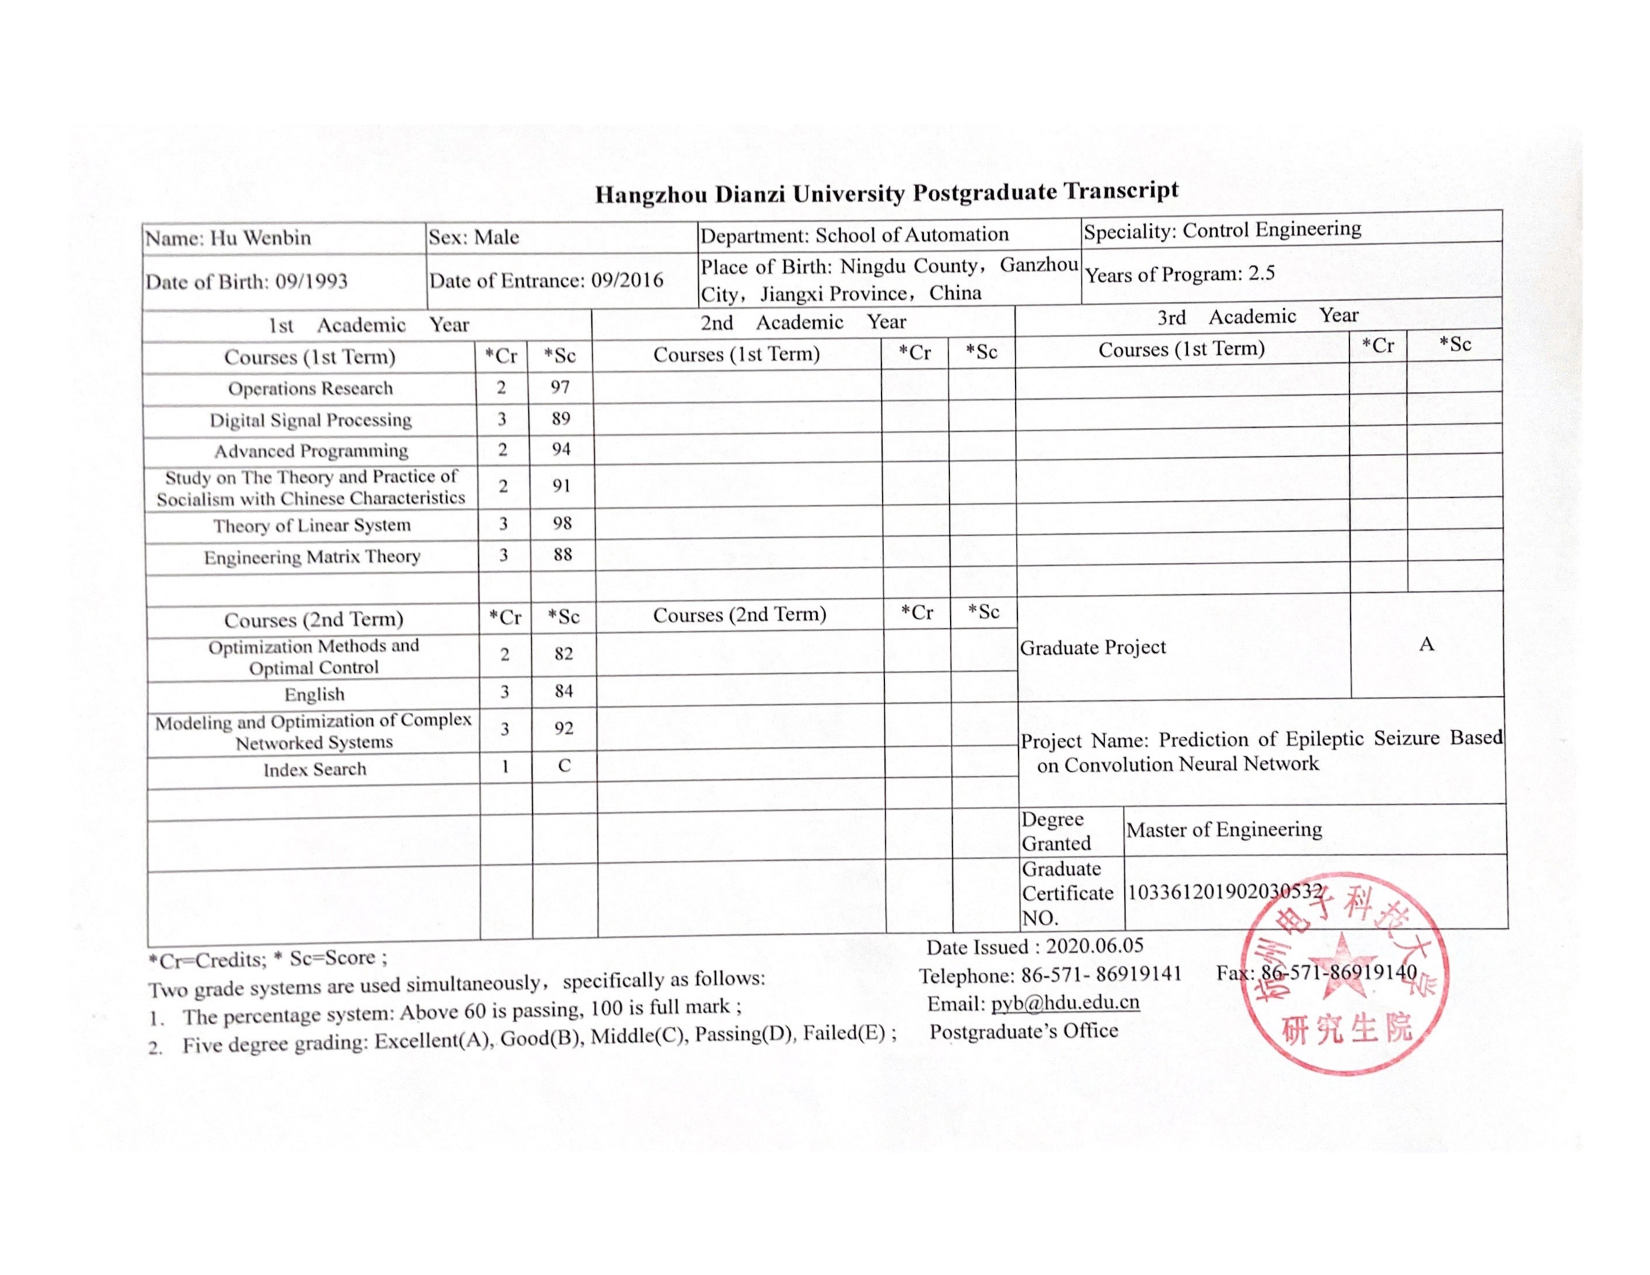
\includepdf[pages=-,pagecommand={},width=1.3\textwidth]{Exhibits/Graduate transcript.pdf}


\vspace*{\fill}
\begin{center}

{\LARGE \bf
Exhibit 4
}

\vspace{10\baselineskip}

{\large Letter of Professor B, University of B}

\end{center}
\vspace*{\fill}


% \includepdf[pages=-,pagecommand={},width=1.3\textwidth]{Exhibits/recomendations/B.pdf}



\vspace*{\fill}
\begin{center}

{\LARGE \bf
Exhibit 5
}

\vspace{10\baselineskip}

{\large  Letter of Dr. C, Lab}

\end{center}
\vspace*{\fill}


% \includepdf[pages=-,pagecommand={},width=1.2\textwidth]{Exhibits/recomendations/C.pdf}




\vspace*{\fill}
\begin{center}

{\LARGE \bf
Exhibit 6
}

\vspace{10\baselineskip}

{\large Letter of Dr. D, University of D}

\end{center}
\vspace*{\fill}

% \includepdf[pages=-,pagecommand={},width=1.3\textwidth]{Exhibits/recomendations/D.pdf}




\vspace*{\fill}
\begin{center}

{\LARGE \bf
Exhibit 7
}

\vspace{10\baselineskip}

{\large Letter of Professor E, University of E}

\end{center}
\vspace*{\fill}

% \includepdf[pages=-,pagecommand={},width=1.3\textwidth]{Exhibits/recomendations/E.pdf}




\vspace*{\fill}
\begin{center}

{\LARGE \bf
Exhibit 8
}

\vspace{10\baselineskip}

{\large Job Offer: University of Whatever}

\end{center}
\vspace*{\fill}


% \includepdf[pages=-,pagecommand={},width=1.3\textwidth]{Exhibits/offer1.pdf}


\vspace*{\fill}
\begin{center}

{\LARGE \bf
Exhibit 9
}

\vspace{10\baselineskip}

{\large Job Offer: Anycompany Inc.}

\end{center}
\vspace*{\fill}

% \includepdf[pages=-,pagecommand={},width=1.3\textwidth]{Exhibits/offer.pdf}




\vspace*{\fill}
\begin{center}

{\LARGE \bf
Exhibit 10
}

\vspace{10\baselineskip}

{\large Bachelor diploma of Mr. Hu}

\end{center}
\vspace*{\fill}

% \includepdf[pages=-,pagecommand={},width=1.3\textwidth]{Exhibits/BSc diploma/BSc diploma english.pdf}

% \includepdf[pages=-,pagecommand={},width=1.3\textwidth]{Exhibits/BSc diploma/BSc diploma original.pdf}


\vspace*{\fill}
\begin{center}

{\LARGE \bf
Exhibit 11
}

\vspace{10\baselineskip}

{\large Graduate degree diploma of Mr. Hu}

\end{center}
\vspace*{\fill}

% \includepdf[pages=-,pagecommand={},width=1.3\textwidth]{Exhibits/PhD diploma/PhDdiploma.pdf}

% \includepdf[pages=-,pagecommand={},width=1.3\textwidth]{Exhibits/PhD diploma/master diploma.pdf}

% \includepdf[pages=-,pagecommand={},width=1.3\textwidth]{Exhibits/PhD diploma/FINAL TRANSCRIPT.pdf}


\vspace*{\fill}
\begin{center}

{\LARGE \bf
Exhibit 12
}

\vspace{10\baselineskip}

{\large Abstract of the Ph.D. dissertation by Mr. Hu}

\end{center}
\vspace*{\fill}


% \includepdf[pages=-,pagecommand={},width=1.3\textwidth]{Exhibits/Thesis abstract.pdf}



\vspace*{\fill}
\begin{center}

{\LARGE \bf
Exhibit 13
}

\vspace{10\baselineskip}

{\large  First pages of 12 papers co-authored by Mr. Hu}

\end{center}
\vspace*{\fill}


% \includepdf[pages=-,pagecommand={},width=1.3\textwidth]{Exhibits/my papers/1.pdf}

% \includepdf[pages=-,pagecommand={},width=1.3\textwidth]{Exhibits/my papers/2.pdf}

% \includepdf[pages=-,pagecommand={},width=1.3\textwidth]{Exhibits/my papers/Thesis.pdf}

% \includepdf[pages=-,pagecommand={},width=1.3\textwidth]{Exhibits/my papers/3.pdf}

% \includepdf[pages=-,pagecommand={},width=1.3\textwidth]{Exhibits/my papers/4.pdf}

% \includepdf[pages=-,pagecommand={},width=1.3\textwidth]{Exhibits/my papers/5.pdf}

% \includepdf[pages=-,pagecommand={},width=1.3\textwidth]{Exhibits/my papers/6.pdf}

% \includepdf[pages=-,pagecommand={},width=1.3\textwidth]{Exhibits/my papers/7.pdf}

% \includepdf[pages=-,pagecommand={},width=1.3\textwidth]{Exhibits/my papers/8.pdf}

% \includepdf[pages=-,pagecommand={},width=1.3\textwidth]{Exhibits/my papers/9.pdf}

% \includepdf[pages=-,pagecommand={},width=1.3\textwidth]{Exhibits/my papers/10.pdf}

% \includepdf[pages=-,pagecommand={},width=1.3\textwidth]{Exhibits/my papers/11.pdf}


\vspace*{\fill}
\begin{center}

{\LARGE \bf
Exhibit 14
}

\vspace{10\baselineskip}

{\large Conference invitations for Mr. Hu}

\end{center}
\vspace*{\fill}

% \includepdf[pages=-,pagecommand={},width=1.3\textwidth]{Exhibits/presentation notifications/ paper notification.pdf}

% \includepdf[pages=-,pagecommand={},width=1.3\textwidth]{Exhibits/presentation notifications/ presentation notification.pdf}

% \includepdf[pages=-,pagecommand={},width=1.3\textwidth]{Exhibits/presentation notifications/C.pdf}

% \includepdf[pages=-,pagecommand={},width=1.3\textwidth]{Exhibits/presentation notifications/A.pdf}

% \includepdf[pages=-,pagecommand={},width=1.3\textwidth]{Exhibits/presentation notifications/CC.pdf}


\vspace*{\fill}
\begin{center}

{\LARGE \bf
Exhibit 15
}

\vspace{10\baselineskip}

{\large Citation reports for Mr. Hu’s papers}

\end{center}
\vspace*{\fill}

% \includepdf[pages=-,pagecommand={},width=1.3\textwidth]{Exhibits/citation reports/blabla.pdf}


\vspace*{\fill}
\begin{center}

{\LARGE \bf
Exhibit 16
}

\vspace{10\baselineskip}

{\large  Review assignments completed by Mr. Hu}

\end{center}
\vspace*{\fill}

% \includepdf[pages=-,pagecommand={},width=1.3\textwidth]{Exhibits/review invites/1 x3.pdf}

% \includepdf[pages=-,pagecommand={},width=1.3\textwidth]{Exhibits/review invites/2.pdf}

% \includepdf[pages=-,pagecommand={},width=1.3\textwidth]{Exhibits/review invites/3.pdf}

% \includepdf[pages=-,pagecommand={},width=1.3\textwidth]{Exhibits/review invites/4.pdf}

% \includepdf[pages=-,pagecommand={},width=1.3\textwidth]{Exhibits/review invites/I5.pdf}

% \includepdf[pages=-,pagecommand={},width=1.3\textwidth]{Exhibits/review invites/I6.pdf}

% \includepdf[pages=-,pagecommand={},width=1.3\textwidth]{Exhibits/review invites/C7.pdf}

% \includepdf[pages=-,pagecommand={},width=1.3\textwidth]{Exhibits/review invites/A8.pdf}

% \includepdf[pages=-,pagecommand={},width=1.3\textwidth]{Exhibits/review invites/A9.pdf}

% \includepdf[pages=-,pagecommand={},width=1.3\textwidth]{Exhibits/review invites/A10.pdf}

% \includepdf[pages=-,pagecommand={},width=1.3\textwidth]{Exhibits/review invites/A11.pdf}

% \includepdf[pages=-,pagecommand={},width=1.3\textwidth]{Exhibits/review invites/A12.pdf}



\vspace*{\fill}
\begin{center}

{\LARGE \bf
Exhibit 17
}

\vspace{10\baselineskip}

{\large Admission letters from graduate schools to Mr. Hu}

\end{center}
\vspace*{\fill}

% \includepdf[pages=-,pagecommand={},width=1.3\textwidth]{Exhibits/admission letters from graduate schools/award notification.pdf}

% \includepdf[pages=-,pagecommand={},width=1.3\textwidth]{Exhibits/admission letters from graduate schools/Fellowship award.pdf}

% \includepdf[pages=-,pagecommand={},width=1.3\textwidth]{Exhibits/admission letters from graduate schools/Letter of Admission.pdf}

% \includepdf[pages=-,pagecommand={},width=1.3\textwidth]{Exhibits/admission letters from graduate schools/email of admission.pdf}

\vspace*{\fill}
\begin{center}

{\LARGE \bf
Exhibit 18
}

\vspace{10\baselineskip}

{\large Announcement of the Assistant Professor position offered to Mr. Hu}

\end{center}
\vspace*{\fill}

% \includepdf[pages=-,pagecommand={},width=1.3\textwidth]{Exhibits/search ad.pdf}


\vspace*{\fill}
\begin{center}

{\LARGE \bf
Exhibit 19
}

\vspace{10\baselineskip}

{\large Occupational Employment and Wage Statistics by U.S. Bureau of Labor Statistics}

\end{center}
\vspace*{\fill}

% \includepdf[pages=-,pagecommand={},width=1.3\textwidth]{Exhibits/salary stats/Computer and Information Research Scientists.pdf}

% \includepdf[pages=-,pagecommand={},width=1.3\textwidth]{Exhibits/salary stats/Electrical Engineers.pdf}

% \includepdf[pages=-,pagecommand={},width=1.3\textwidth]{Exhibits/salary stats/Operations Research Analysts.pdf}

% \includepdf[pages=-,pagecommand={},width=1.3\textwidth]{Exhibits/salary stats/Industrial Engineers.pdf}




\vspace*{\fill}
\begin{center}
{\LARGE \bf
Exhibit 20
}

\vspace{10\baselineskip}

{\large Academic Ranking of World Universities 2024}

\end{center}
\vspace*{\fill}

 \includepdf[pages=-,pagecommand={},width=1.3\textwidth]{Exhibits/Academic Ranking of World Universities 2024.pdf}

\vspace*{\fill}
\begin{center}
{\LARGE \bf
Exhibit 21
}

\vspace{10\baselineskip}

{\large Statistical Bulletin on the Development of National Education in China}

\end{center}
\vspace*{\fill}

\includepdf[pages=-,pagecommand={},width=1.3\textwidth]{Exhibits/Statistical Bulletin on the Development of National Education in China.pdf}


\vspace*{\fill}
\begin{center}
{\LARGE \bf
Exhibit 22
}

\vspace{10\baselineskip}

{\large University of Anywhere page on the website of Carnegie Classification\\ of Institutions of Higher Education}

\end{center}
\vspace*{\fill}


% \includepdf[pages=-,pagecommand={},width=1.3\textwidth]{Exhibits/doc.pdf}



\vspace*{\fill}
\begin{center}
{\LARGE \bf
Exhibit 23
}

\vspace{10\baselineskip}

{\large USNews article on top AI technology stocks}

\end{center}
\vspace*{\fill}


% \includepdf[pages=-,pagecommand={},width=1.3\textwidth]{Exhibits/US news top AI companies.pdf}



\vspace*{\fill}
\begin{center}
{\LARGE \bf
Exhibit 24
}

\vspace{10\baselineskip}

{\large Top venues in Artificial Intelligence, Mathematical Optimization, and Power Engineering}

\end{center}
\vspace*{\fill}


% \includepdf[pages=-,pagecommand={},width=1.3\textwidth]{Exhibits/Top Venues/Artificial Intelligence - Google Scholar Metrics.pdf}

% \includepdf[pages=-,pagecommand={},width=1.3\textwidth]{Exhibits/Top Venues/Journal Rankings on Artificial Intelligence.pdf}

% \includepdf[pages=-,pagecommand={},width=1.3\textwidth]{Exhibits/Top Venues/Mathematical Optimization - Google Scholar Metrics.pdf}

% \includepdf[pages=-,pagecommand={},width=1.3\textwidth]{Exhibits/Top Venues/Power Engineering - Google Scholar Metrics.pdf}



\vspace*{\fill}
\begin{center}
{\LARGE \bf
Exhibit 25
}

\vspace{10\baselineskip}

{\large Description of the Grid Modernization and the Smart Grid project by the Department of Energy}

\end{center}
\vspace*{\fill}

\includepdf[pages=-,pagecommand={},width=1.3\textwidth]{Exhibits/Grid Modernization and the Smart Grid _ Department of Energy.pdf}




\vspace*{\fill}
\begin{center}
{\LARGE \bf
Exhibit 26
}

\vspace{10\baselineskip}

{\large The White House Greenhouse Gas Pollution Reduction Target}

\end{center}
\vspace*{\fill}

\includepdf[pages=-,pagecommand={},width=1.3\textwidth]{Exhibits/the White House Greenhouse Gas Pollution Reduction Target.pdf}




\vspace*{\fill}
\begin{center}
{\LARGE \bf
Exhibit 27
}

\vspace{10\baselineskip}

{\large The description of Clean Energy Initiative by the State Energy Office }

\end{center}
\vspace*{\fill}

% \includepdf[pages=-,pagecommand={},width=1.3\textwidth]{Exhibits/doc.pdf}




\vspace*{\fill}
\begin{center}

{\LARGE \bf
Exhibit 28
}

\vspace{10\baselineskip}

{\large The page devoted to Artificial Intelligence (AI) by the U. S. Department of State}

\end{center}
\vspace*{\fill}

\includepdf[pages=-,pagecommand={},width=1.3\textwidth]{Exhibits/Artificial Intelligence (AI) - United States Department of State.pdf}




\vspace*{\fill}
\begin{center}

{\LARGE \bf
Exhibit 29
}

\vspace{10\baselineskip}

{\large New Actions to Promote Responsible AI Innovation that Protects Americans’ Rights and Safety}

\end{center}
\vspace*{\fill}

\includepdf[pages=-,pagecommand={},width=1.3\textwidth]{Exhibits/AI Biden-Harris Administration Announces New Actions to Promote Responsible AI Innovation.pdf}




\vspace*{\fill}
\begin{center}

{\LARGE \bf
Exhibit 30
}

\vspace{10\baselineskip}

{\large W-2 form Mr. Hu received from Anycompany Inc. for the calendar year 2022}

\end{center}
\vspace*{\fill}

% \includepdf[pages=-,pagecommand={},width=1.2\textwidth]{Exhibits/W2.pdf}





\end{document}
